\chapter{Introduction}
\label{chap:introduction}

The evolution of technology is inherently bound to the evolution of society and human desires. In recent years the focus of the technology-mediated services has shifted from mere functionalism to become more aesthetically, functionally, socially, and interactively pleasurable. The most successful multimedia creation and distribution companies offer customized recommending services and then aggregate correct predictions between users sharing similar taste or preferences to improve their offer: an experience as tailored as possible to users' individual needs. Understanding users’ behavior and emotions is not only very profitable for companies that want to continuously engage their users, but also a popular topic among researchers and designers that thrive to better understand the human mind to enhance the quality of human-computer interactions. It is also becoming a necessity for the end users themselves, who are not satisfied anymore by tinkering with technology but want the interaction to be flexible and seamlessly usable in the daily life. Recent applications and services offer the possibility for people to monitor their body, mind, and health through continuous collection of physiological signals from wearable sensors, for example to keep track of good sport habits, sleep quality, stress level and more. But it is also possible to infer affective states from clues in the recorded brain activity. Given the increasing interest of researchers and companies in the affective field, the more and more frequent use of physiological and behavioral clues to assess mental states will keep growing until technologies of daily use will be standardly designed with brain-reading capabilities. The human brain is the central and most important organ of our body because it is where our consciousness, our “self”, resides and it is the command center of all vital functions. And yet, it is also the one we understand least, despite the ongoing research. We rightfully assume emotions originate in the brain, but we can only observe their physiological responses and we can only qualitatively support these observations through inherently imprecise self-assessment tools. Trying to find a correlation between the physiological response and the self-assessed mental state or emotion is not as simple as correlating factual measures, because of the uncertainty of the factors involved. Modern wearable \ac{BCIs}, mostly represented by EEG-capable devices, are still limited in their functionalities and design. Recorded signals are often affected by noise or artifactual information and the user experience is so heavily hindered that most companies are reluctant in investing into them, and more research and optimization is needed before pushing them to the general public. Self-assessing emotions is also non-trivial because it requires a strong understanding of one’s perceived emotions, and this perception has great variability from individual to individual. Creating models able to generalize through all the subjective differences is complicated, especially with performances that enable designers to create enjoyable user experiences for everyone. Thus, we enter in a challenging and almost paradoxical situation: on one hand the goal is to find a common approach to exploit generic behavioral and physiological patterns, on the other hand it is also necessary to account for individual differences to offer the customized experience that users desire. This research takes an extra step into the challenge by evaluating what could be the classification performances of an affective \ac{BCI} system for emotion-aware recommendations using a wearable device. It delves on relevant insights on the main problematics that researchers and designers will face in the years to come when classifying brain emotions, and finally discusses possible solutions and future developments towards online Emotion-Recognition.

\section{Motivation}
\label{sec:motivation}
In 2016, the American research and advisory information firm Gartner published their yearly hype cycle for emerging 
technologies , positioning “Brain-Computer Interfaces” and “Affective Computing” on the growing slope of the “Peak of Inflated Expectations”, both with an estimated period of about 10 or more years before mainstream adoption (see Figure \ref{fig_hype_cycle}).
\begin{figure}[ht]
%Insert your figure here. Make sure that the type of figure file (eps/pdf/...) complies with your typesetter.
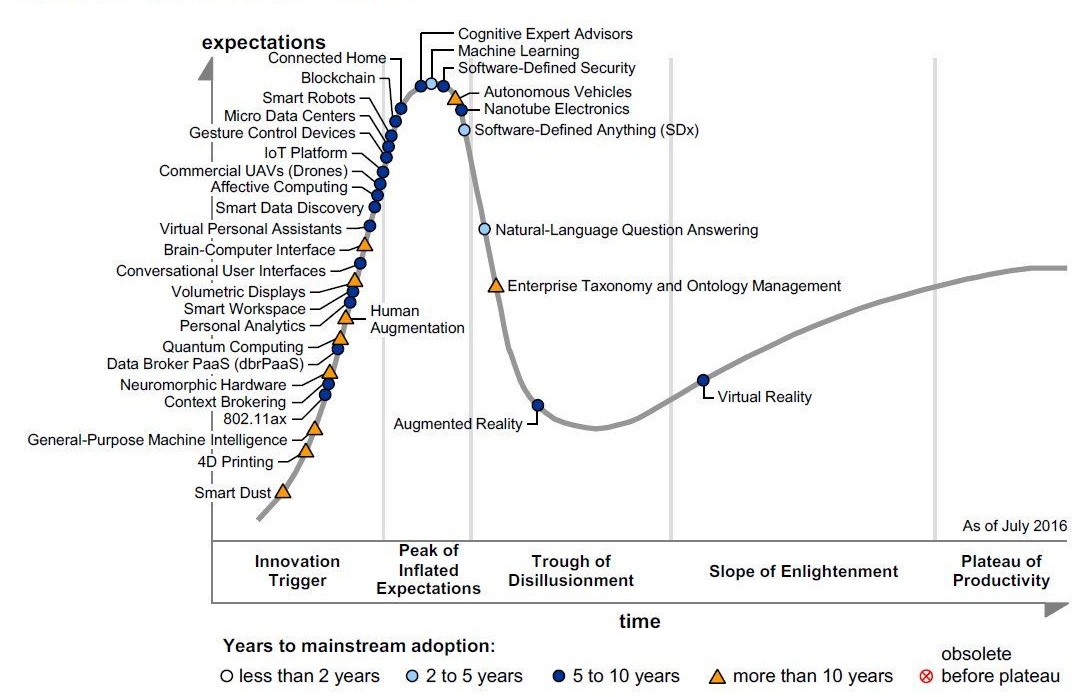
\includegraphics[width=\textwidth]{img/intro/hype_curve_trim.jpg}
\caption{Gartner hype cycle for emerging technologies in 2016, from Gartner\cite{noauthor_gartners_nodate}}\label{fig_hype_cycle}
\end{figure}
In the versions published over the last 5 years, "Affective Computing" completely disappeared from the hype cycle and "Brain-Computer Interfaces" slowly climbed the slope before disappearing as well. This trend suggests that both fields reached the peak of the inflated expectations and fell down the “Through of Disillusionment” slope as the technology failed to meet the expectations of users, researchers, and investors. Nevertheless, some innovative companies and startups stepped up to the challenge and started a new innovation cycle by developing wearable neural sensors and slowly pushing again \ac{BCI} towards mainstream adoption. For example, NextMind\footnote{https://www.next-mind.com/}  released in early 2021 a wearable sensor for active control of multimedia applications and games. Muse\footnote{https://choosemuse.com/} instead developed several wearable \ac{BCIs} for neurofeedback during guided meditations, recently updated to be used for sleep tracking. Enophone produces EEG-capable headphones and recently made a partnership with BrainFlow to integrate their SDK and build affective applications for music listening \cite{parfenov_brainflow_nodate}. Melomind\footnote{https://www.melomind.com/en/product/melomind-en/} , the device used in the current research, is another EEG capable device with headphones and an application for neurofeedback training. Ontbo\footnote{https://ontbo.com/en/} already promises an application with their headphones to generate music playlists that can alter the level of motivation, relaxation, stress, and concentration in the brain activity. Major brands like Valve, Tobii and OpenBCI are collaborating to bring together the world of virtual reality and \ac{BCI} \cite{parfenov_openbci_nodate}, and Facebook is developing their own neural interfaces after acquiring the neurotech startup CTRL-Labs \cite{statt_facebook_2019}. In the academic world, we can find very recent papers that focused on affective music recommendations, for example Chang et al. \cite{chang_personalized_2017} proposed a recommending system to suggest the appropriate stress-relief music to the users based on the inferred stress level in their EEG, while Abdul et al. \cite{abdul_emotion-aware_2018} designed an emotion-aware system to correlate implicit emotional user tags and musical features. This reignited interest in affective applications and the development of a new generation of \ac{BCIs} supports the relevance in researching and developing now the methods and tools that will be used to design the affective systems of tomorrow. Given this context, music is one of the best elicitors for the field of Emotion-Recognition for a multitude of reasons: 
\begin{itemize}
\item It is a proven powerful elicitor that arouses instinctive physiological reactions in the human body.
\item It has been used for centuries to convey emotional meaning, and now more than ever even across cultures, social classes, and age groups.
\item The physiological emotional response is agnostic of the stimulus, thus findings on music-elicited Emotion-Recognition are theoretically transferrable to other applications.
\item The market of music recommending systems is flourishing and very competitive, with many companies taking part in the technological development of such systems.
\end{itemize}
The music-emotion experience is very personal and influenced by internal factors, such as tempo and pitch of a song, as well as external factors such as memories, context, or correlated events associated to a past pleasurable or unpleasurable experience. 
The proposal of this study is a novel approach to the Emotion-Recognition task using Melomind, a wearable and consumer-oriented \ac{BCI}. The goal is to investigate the feasibility and the performances of the classification task in realistic listening conditions to evaluate the future development of wearable \ac{BCIs} equipped with online Emotion-Recognition for daily use. Instead of focusing on the correlation between the musical features and the \ac{ERPs} in the brain, the approach of this research is to use emotion-labelled songs as elicitors to study the spectral properties of frequency bands associated with emotions in the \ac{EEG} signal. These spectral properties can be translated into features and used for the computation of neural biomarkers, called “neuromarkers” in this research, to be fed into a classifier for the classification of the emotional valence and arousal based on known patterns in the brain activity. To support the collected physiological data, participants have been asked to continuously self-assess their emotions in a coordinate system representing the emotional dimensions of valence and arousal. The research questions of this study try to fulfil the design requirements of exploring the performances of the Emotion-Recognition task using a wearable \ac{EEG}  headset, considering the disadvantages and the advantages of this specific technology. The dry electrodes of the Melomind in pair with the headphones form factor allow for a very quick and relatively comfortable setup, enabling the researcher to focus on the task and overall shorten the experimental sessions. Consequently, it was possible for a single researcher to collect data from 45 subjects over 15 days. This technology has also limited recording capabilities; thus, the quality and quantity of data is lower than what could be obtained with standard \ac{EEG} lab equipment featuring 32 wet electrodes headcaps. Furthermore, the position of the Melomind electrodes only allows recording signals from the frontal and/or the parietal regions of the cerebral cortex, limiting considerably the area of study. The data has been collected through an experimental phase as result of a collaboration between the University of Twente and myBrainTechnologies, the company that manufactures Melomind. The research was approved by the Ethics Committee Computer \& Information Science and the Dean of the EEMCS  faculty following the regulations in force at the University of Twente, with reference number RP 2021-43.


\section{Research questions}
\label{sec:goal}
To evaluate this novel approach, this study aims to answer the following main research question:
\\
\\
\textbf{RQ}: \emph{ “What are the accuracy and MCC scores of subject-dependent classification of music-elicited emotional valence and arousal in the EEG signal using SVM and MLP algorithms with Melomind?”}
\\
\\
The mains research question was then extended by the following sub questions to support possible design choices for a real-time music recommending system based on brain activity.
\\
\\
\textbf{SRQ1}: \emph{“What are the most relevant selected Power Spectral Density features to perform the Emotion-Recognition using SVM and MLP algorithms with Melomind?”}
\\
\\
\textbf{SRQ2}: \emph{“What is the best classification strategy applicable to the current software and hardware capabilities of Melomind using SVM and MLP algorithms?”}



\section{Report organization}
\label{sec:organization}
To answer these research questions, the main models for self-assessment of emotions have been studied, together with the existing models relating the two main dimensions of emotional valence and arousal to brain activity (see Chapter \ref{chap:background}). The most compelling related work in classification of music-elicited emotions has been reviewed (see Chapter \ref{chap:related_work}) and used as methodical foundation. An experiment was designed to collect data in two listening conditions  and a processing pipeline was implemented to extract features and to train classification algorithms that could produce comparable results with the related work (see Chapter \ref{chap:methods}). The results were then collected (see Chapter \ref{chap:results}) and discussed with a view to possible future developments (see Chapter \ref{chap:discussion}).